\documentclass[11pt,letterpaper]{article}
\PassOptionsToPackage{hyphens}{url}
\usepackage[margin=.83in,top=.8in,bottom=.8in,headheight=15pt]{geometry}
\usepackage[T1]{fontenc}
\usepackage{lmodern,amsmath,amssymb,mathtools,bm,booktabs,array,graphicx,tikz}
\usetikzlibrary{arrows.meta,positioning,calc,decorations.pathreplacing,patterns}
\definecolor{ink}{HTML}{17344D}\definecolor{accent}{HTML}{087E8B}\definecolor{pale}{HTML}{EDF5F5}\definecolor{gold}{HTML}{AD6B19}
\providecommand{\dd}{\,\mathrm{d}}\providecommand{\R}{\mathbb{R}}
\providecommand{\E}{\mathbb{E}}\providecommand{\Var}{\operatorname{Var}}
\providecommand{\Cov}{\operatorname{Cov}}\providecommand{\diag}{\operatorname{diag}}
\providecommand{\norm}[1]{\left\lVert#1\right\rVert}
\providecommand{\abs}[1]{\left|#1\right|}
\usepackage{microtype,hyperref,fancyhdr,enumitem,amsthm,sectsty,needspace}
\allsectionsfont{\raggedright}
\hypersetup{colorlinks=true,linkcolor=ink,urlcolor=accent,pdfauthor={Zan Ahmad},pdftitle={Neural-network gradients and spatial filters / Lecture notes}}
\setlength{\parindent}{0pt}\setlength{\parskip}{6pt}\linespread{1.07}
\setlist{itemsep=3pt,topsep=4pt,leftmargin=*}
\emergencystretch=2em\clubpenalty=10000\widowpenalty=10000
\pagestyle{fancy}\fancyhf{}\fancyhead[L]{\small Scientific Computing in Python / 2027}\fancyhead[R]{\small Lecture 5}
\fancyfoot[L]{\footnotesize Zan Ahmad}\fancyfoot[R]{\footnotesize\thepage}\renewcommand{\headrulewidth}{.3pt}
\newtheorem{proposition}{Proposition}\newtheorem{theorem}{Theorem}\newtheorem{lemma}{Lemma}
\theoremstyle{definition}\newtheorem{definition}{Definition}\newtheorem{example}{Example}
\numberwithin{equation}{section}
\begin{document}
{\small\scshape Scientific Computing in Python / 2027\hfill Lecture 5}\par\medskip
{\raggedright\hyphenpenalty=10000\exhyphenpenalty=10000\LARGE\bfseries\color{ink} Neural-network gradients and spatial filters\par}\medskip
{\small Lecture notes}\par\bigskip
An image is an array of measured intensities. We first treat that array as a vector and derive the forward and backward passes of a small neural network. We then retain its spatial structure and apply local filters. The synthetic stripe problem makes both computations explicit, while keeping the distinction between fixed filters and learned parameters visible.

\section{Images as arrays}
\hypertarget{note-images-as-arrays}{}\label{note:images-as-arrays}
{\small \href{slides.html\#frame=images-as-arrays\&step=1}{Slides for this section}}\par
An $8\times8$ single-channel image contains 64 scalar intensities. Flattening produces a vector with a fixed ordering. The ordering does not discard numerical entries, but a dense layer does not explicitly encode which pixels are adjacent. A local filter uses spatial indices to reuse the same coefficients across positions.

\[
X\in\R^{n\times8\times8\times1},\qquad
X_{\rm flat}\in\R^{n\times64}.
\]

Flattening preserves the values and fixes a coordinate convention.

\subsection*{An affine hidden layer}
\[
U=X_{\rm flat}W_1+b_1,\quad H=\tanh U,
\]

\[
z=Hw_2+b_2,\qquad p=\sigma(z).
\]
For $h$ hidden units, $W_1$ has shape $64\times h$.
\section{The binary loss}
\hypertarget{note-the-binary-loss}{}\label{note:the-binary-loss}
{\small \href{slides.html\#frame=the-binary-loss\&step=1}{Slides for this section}}\par
For binary labels the negative Bernoulli log likelihood can be written in terms of logits. This avoids directly taking logarithms of scores that have rounded to zero or one. Averaging over the training batch makes the data term's scale independent of batch length.

\[
L=\frac1n\sum_i[\log(1+e^{z_i})-y_iz_i].
\]

\begin{minipage}{\linewidth}
\begin{verbatim}
loss = np.mean(np.logaddexp(0, z) - y*z)
\end{verbatim}
\end{minipage}

\subsection*{Derivative with respect to the logits}
\[
\frac{\partial L}{\partial z_i}=\frac{p_i-y_i}{n}.
\]

The derivative is bounded even when a logit has large magnitude. Stable evaluation remains necessary.
\section{Backpropagation}
\hypertarget{note-backpropagation}{}\label{note:backpropagation}
{\small \href{slides.html\#frame=backpropagation\&step=1}{Slides for this section}}\par
The chain rule propagates the loss derivative from logits to hidden states and then to the first affine map. Tanh has derivative $1-H^2$, applied entrywise. Matrix shapes expose which indices are being summed. Penalty terms, if included in the objective, contribute additional parameter derivatives.

Let $D=(p-y)/n$. Then
\[
\nabla_{w_2}L=H^{\mathsf T}D,\qquad D_1=(Dw_2^{\mathsf T})\odot(1-H^2).
\]

\[
\nabla_{W_1}L=X_{\rm flat}^{\mathsf T}D_1.
\]

\subsection*{A finite-difference gradient check}
For a parameter coordinate $\theta_j$,
\[
\partial_jL\approx\frac{L(\theta+\epsilon e_j)-L(\theta-\epsilon e_j)}{2\epsilon}.
\]

Use a moderate $\epsilon$: too large gives truncation error, too small gives cancellation error.
\begin{center}\begin{minipage}{.98\linewidth}\centering
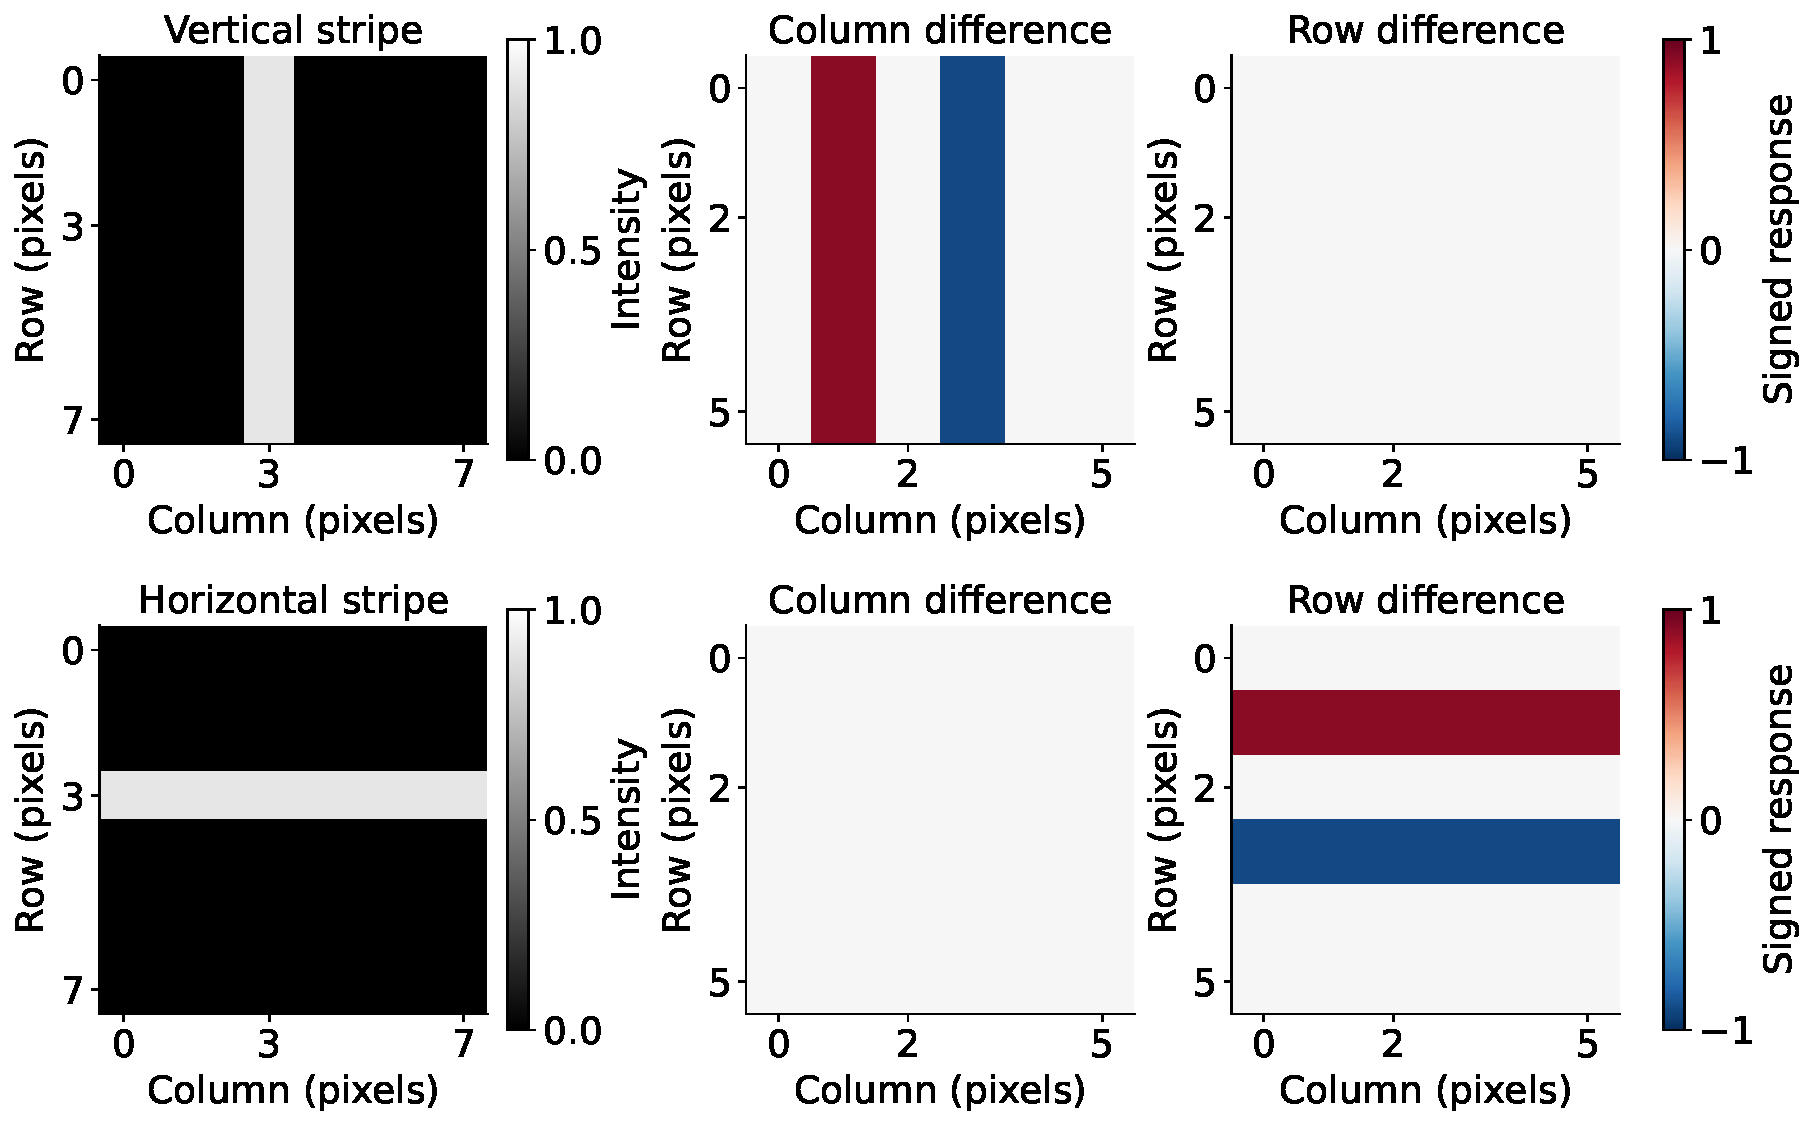
\includegraphics[width=.96\linewidth,height=.57\textheight,keepaspectratio]{presentation-figures/filters.pdf}\par\smallskip
{\small Separate idealized 8$\times$8 display images place each stripe in the interior so both edge signs remain visible in the 6$\times$6 responses. These fixed 3$\times$3 filters use cross-correlation with no padding; red and blue show opposite signs. The images are not benchmark samples, and the filters are not learned.}
\end{minipage}\end{center}
\section{Local cross-correlation}
\hypertarget{note-local-cross-correlation}{}\label{note:local-cross-correlation}
{\small \href{slides.html\#frame=filters-panel-1\&step=1}{Slides for this section}}\par
A $3\times3$ filter applied without padding to an $8\times8$ image produces a $6\times6$ response. The implemented operation is cross-correlation because it does not reverse the filter indices. Deep-learning libraries often call this operation convolution. Its boundary convention must be stated because padding changes both shape and edge behavior.

\[
R_{nijf}=\sum_{u=0}^{2}\sum_{v=0}^{2}X_{n,i+u,j+v,0}K_{uv0f}.
\]

The output shape is $(n,6,6,F)$ for $F$ filters.

\subsection*{Output size}
For input width $W$, filter width $k$, padding $p$, and stride $s$,
\[
W_{\rm out}=\left\lfloor\frac{W+2p-k}{s}\right\rfloor+1.
\]

Here $W=8$, $k=3$, $p=0$, $s=1$, giving $6$.
\section{Filter response and orientation}
\hypertarget{note-filter-response-and-orientation}{}\label{note:filter-response-and-orientation}
{\small \href{slides.html\#frame=filter-response-and-orientation\&step=1}{Slides for this section}}\par
A filter with coefficients summing to zero gives zero response on a constant patch. A signed edge filter responds differently to increasing and decreasing intensity. Reversing the edge reverses the sign. The filters in this demonstration are fixed by construction, while the dense network parameters are fitted from labeled images.

\[
K=\frac13\begin{pmatrix}-1&0&1\\-1&0&1\\-1&0&1\end{pmatrix},\qquad \sum_{u,v}K_{uv}=0.
\]

A constant patch has response $c\sum K_{uv}=0$.

\subsection*{Parameter sharing}
The same $3\times3$ coefficients act at every valid image position.

This reuses nine parameters per input/output channel pair. A dense map would assign separate weights to each input coordinate for each output.

A different pointwise activation, used in the exercises, is the rectified linear unit:
\[
\operatorname{ReLU}(a)=\max(0,a).
\]
It preserves positive responses and sets negative responses to zero. In contrast, $|a|$ preserves the magnitude of both signs. Thus applying ReLU to a signed edge response discards one edge orientation; taking its absolute value treats the two orientations alike. The fitted network in the companion uses $\tanh$, not ReLU; these are alternative activation choices.
\begin{center}\begin{minipage}{.98\linewidth}\centering
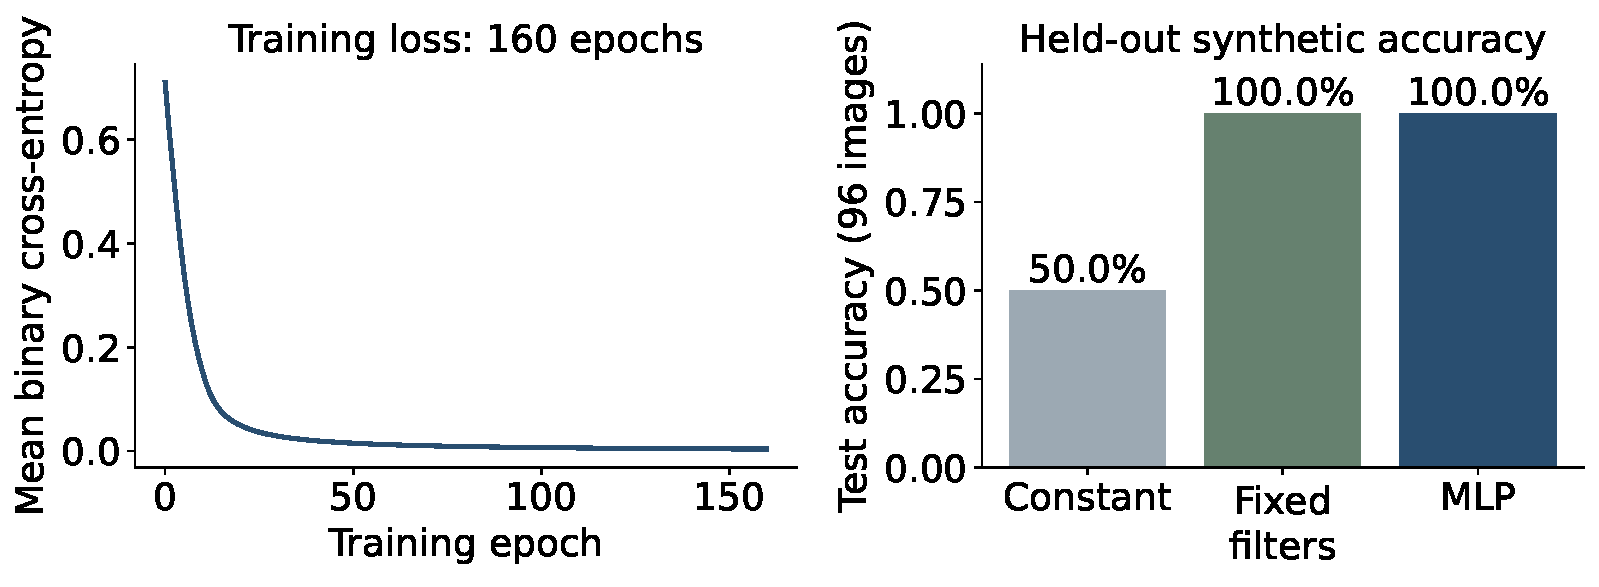
\includegraphics[width=.96\linewidth,height=.57\textheight,keepaspectratio]{presentation-figures/learning-and-baselines.pdf}\par\smallskip
{\small Computed deterministic results: training loss decreases over 160 epochs; test accuracy is 50\% for the constant baseline and 100\% for both the fixed-filter rule and the small trained MLP. All 96 test images come from the same synthetic generator family.}
\end{minipage}\end{center}
\section{Baselines and generalization}
\hypertarget{note-baselines-and-generalization}{}\label{note:baselines-and-generalization}
{\small \href{slides.html\#frame=learning-and-baselines-figure\&step=1}{Slides for this section}}\par
A constant classifier and a fixed-filter rule establish what can be achieved without training a neural network. The supplied synthetic experiment is simple enough that both a suitable fixed rule and the small fitted network can classify its held-out generator samples perfectly. This result does not establish robustness to new acquisition processes, rotations, artifacts, or biological images.

The comparison holds the training/test split fixed and evaluates
\[
\text{constant rule},\quad\text{fixed spatial filter},\quad\text{trained network}.
\]

A higher-capacity model is useful only if it improves the relevant task.

\subsection*{Distribution shift}
A test set drawn from the same generator checks interpolation within that experiment.

A changed generator tests a different claim. Specify which image transformations and noise changes are included before evaluating robustness.
\bigskip
\section*{Exercises}
\par\noindent\begin{minipage}{\linewidth}
\subsection*{N5-1. Trace a tiny network}
For one example, x=\allowbreak{}[2, 1]. Use first-layer weight rows [1, -1] and [0.5, 1], bias [-1, 0], then ReLU. The output weights are [2, -1], output bias -2, and sigmoid gives the class 1 probability.

\textbf{a} Compute the two first-layer values and the ReLU activations.

\end{minipage}\par\medskip
\textbf{b} Compute the logit and approximate probability.

\textbf{c} If the label is 1, what is the output-bias gradient for this one example, and which direction does gradient descent move it?

\par\noindent\begin{minipage}{\linewidth}
\subsection*{N5-2. Shapes and shared parameters}
A batch contains 5 single-channel 8$\times$8 images. Apply two 3$\times$3 filters at stride 1 without padding.

\textbf{a} State the input, filter and output shapes using the lesson's axis order.

\end{minipage}\par\medskip
\textbf{b} How many learned parameters would two such filters have if each had one learned bias? How many are learned in the fixed-filter demonstration?

\textbf{c} What shape remains after averaging absolute responses across both spatial axes? What distinction does ReLU make instead?

\par\noindent\begin{minipage}{\linewidth}
\subsection*{N5-3. Evaluate before enlarging the claim}
On 80 held-out examples, a model has confusion counts [[36, 4], [10, 30]], with true classes in rows and predicted classes in columns. Both true classes contain 40 examples.

\textbf{a} Compute accuracy and class 1 recall.

\end{minipage}\par\medskip
\textbf{b} Compare with a constant baseline and state one limitation of accuracy alone.

\textbf{c} A student tries ten hidden widths and reports the best score on this same test set. What must change before a final unbiased evaluation?

\par\noindent\begin{minipage}{\linewidth}
\subsection*{N5-4. Check a computation and its limits}
For one parameter w, a loss calculation gives L (w+\allowbreak{}0.001)=\allowbreak{}0.420310 and L (w-0.001)=\allowbreak{}0.419710. The coded derivative is 0.30001.

\textbf{a} Compute the centered finite-difference derivative and its absolute discrepancy from the coded value.

\end{minipage}\par\medskip
\textbf{b} For w=\allowbreak{}0.7 and learning rate 0.05, what update follows from the finite-difference slope?

\textbf{c} A constant-intensity image gives zero response to the two derivative filters. Does that make it a valid vertical or horizontal example?

\section*{References}
\noindent\begin{minipage}{\linewidth}
Original Python Lecture 2. PDF pp. 30--33 and 41: array products and shapes.

\url{https://zanahmad.com/files/scientific-python/Lecture_2__Intro_to_Python.pdf}
\end{minipage}\par\medskip
\noindent\begin{minipage}{\linewidth}
Original derivation and executable checks in this lesson. Sections 2--5 and demo.py: forward map, stable binary loss, gradient check and fixed-filter calculation.

\end{minipage}\par\medskip
Python source materials: Phillip Kerger (2023). Course adaptation and additional exposition: Zan Ahmad.

\end{document}
